\documentclass[10pt,a4paper]{article}
%\usepackage[natbibapa]{apacite} 
\usepackage{enumitem}
\usepackage{tikz}
\usetikzlibrary{automata,positioning}
%\bibliographystyle{apacite}


\title{Natural Language Processing (COS4861)}
\author{Adriaan Louw (53031377)}

\begin{document}

\maketitle

\section{Question 1}
\begin{enumerate}[leftmargin=\labelsep]
\item[1.1]$/[a-zA-Z]?[a-z]*/$

\item[1.2]$/([a-zA-Z]?[a-z]*)\backslash s \backslash 1/$

\item[1.3]$/([a-zA-Z]?[a-z]*)\backslash s [a-zA-Z]?[a-z]* \backslash s \backslash 1/$

\item[1.4.a]This string start off at the beginning of a line.It start with 3 asterisks (*), followed by 2 or 3 pluses (+). That is followed by one colon (:) and a space. That is followed by a string containing upper and lower case letters and the underscore. There will be at least one character in this substring. Then we have another colon. Then the same amount of pluses we had before and to finish this string 9 off we have 3 asterisks. This string will also end the line.

\item[1.4.b] $***++: CompCSI\_\_N\_L\_P\_\_COS\_4861 :++***$ \newline
 (please note there is a space after the first "$:$" and a space before the second "$:$")

\item[1.5] $/0((11)+0)*1*/$

\item[1.6.a] $/\backslash w+(\backslash . \backslash w +)*@ \backslash w+(\backslash . \backslash w +)*$

\item[1.6.b] The initial accuracy was 0.66. \newline
             The RE was then changed to $/\backslash w+([\backslash . \backslash w\backslash ' \backslash -] +)*@ \backslash w+(\backslash . \backslash w +)*$ which has an accuracy of 1 over the training set and it did not match anything but email address's. The data used to determine the correct form of an email address can be found at $https://tools.ietf.org/html/rfc3696$
 
\item[1.7] Accuracy for this training set was 0.66 \newline
 The address richard.j.beatty@mvp02.usace.army.mil was not matched completely because the address was over multiple lines. \newline
 The address "jomose AT abranch DOT com" was not matched because it uses multiple words and does not have the $@$ sign. \newline
 The RE also incorrectly matched the "address" "trailers@residences", which is not an address at all. This is not taken into account in the accuracy calculation      

\item[1.8] We start with $Q' = \{\{1\}\}$ \newline
With $q=\{1\} $ we have $t=\bigcup_{p\epsilon q}\delta(p,0) = \{1\}\cup\{2\}\cup\{3\}\cup\{4\}\cup\{5\} = \{1,2,3,4,5\}$ add t to Q'. Thus $Q'=\{\{1\},\{1,2,3,4,5\}\}$. Then for $t=\bigcup_{p\epsilon q}\delta(p,1) = \{4,5\}$. Then we also add t to Q', making $Q'=\{\{1\},\{1,2,3,4,5\},\{4,5\}\}$. We then also add $\delta(\{1\},0)=\{1,2,3,4,5\}$ and $\delta({1},1)=\{4,5\}$ to $\delta'$. To determine new accepts states we see that $q\cap A = \emptyset$ which means we do not add anything to A'. 

For $q=\{1,2,3,4,5\}$ we get $\delta(\{1,2,3,4,5\},0)=\delta(\{1\},0)\cup\delta(\{2\},0)\cup(\{3\},0)\cup\delta(\{4\},0)\cup\delta(\{5\},0)=\{1,2,3,4,5\}$, which we add to Q', but since it is already in Q' there is no effect. Then $\delta(\{1,2,3,4,5\},1) = \{3,4,5\}$, which means we add $\{3,4,5\}$ to Q'. Thus, $Q'=\{\{1\},\{1,2,3,4,5\},\{4,5\},\{3,4,5\}\}$. Then we add to mappings $\delta(\{1,2,3,4,5\},0)=\{1,2,3,4,5\}$ and $\delta(\{1,2,3,4,5\},1) = \{3,4,5\}$ to $\delta'$. Calculating whether we have a new accept state, we have $q\cap A = \{4\}$. Thus we add $\{1,2,3,4,5\}$ to A'.

For $q=\{4,5\}$, $t=\delta(\{4,5\},0)=\emptyset$. We add $\emptyset$ to Q' and the mapping 
$t=\delta(\{4,5\},0)=\emptyset$ to $\delta'$. Then $t=\delta(\{4,5\},1)=\{4\}$. Which means we add the state $\{4\}$ to Q' and the mapping $\delta(\{4,5\},1)=\{4\}$ to $\delta'$. $q\cap A =\{4\}$, so we add $\{4,5\}$ to A'. Now  $Q'=\{\{1\},\{1,2,3,4,5\},\{4,5\},\{3,4,5\},\{4\},\emptyset\}$.

Next we have $q=\{3,4,5\}$. Or 2 new mappings are $\delta(\{3,4,5\},0)= \{2\}$ and $\delta(\{3,4,5\},1)=\{4\}$, which we add to $\delta'$. Then we only add $\{2\}$ to Q' because $\{4\}$ is already in Q'. For the accept state check we have $q\cap A = \{4\}$. SO we add $\{3,4,5\}$ to A'.

Then for $q=\{2\}$ we have $\delta(\{2\},0)=\emptyset$ and $\delta(\{2\},1) = \{4\}$. These mappings we add to $\delta'$. We also do not add any new states to Q' since the new states are in Q'. Also $q\cap A = \emptyset$ so no new accept states.

The state $\{4\}$ has no outgoing states so we can ignore this state in terms of generating new states.

Now we have gone through all the states in Q'. The result is \newline $Q'=\{\{1\},\{1,2,3,4,5\},\{4,5\},\{3,4,5\}, \{4\},\emptyset\,\{2\}\}$ and \newline $A=\{\{1,2,3,4,5\},\{4,5\},\{3,4,5\},\{4\}\}$.

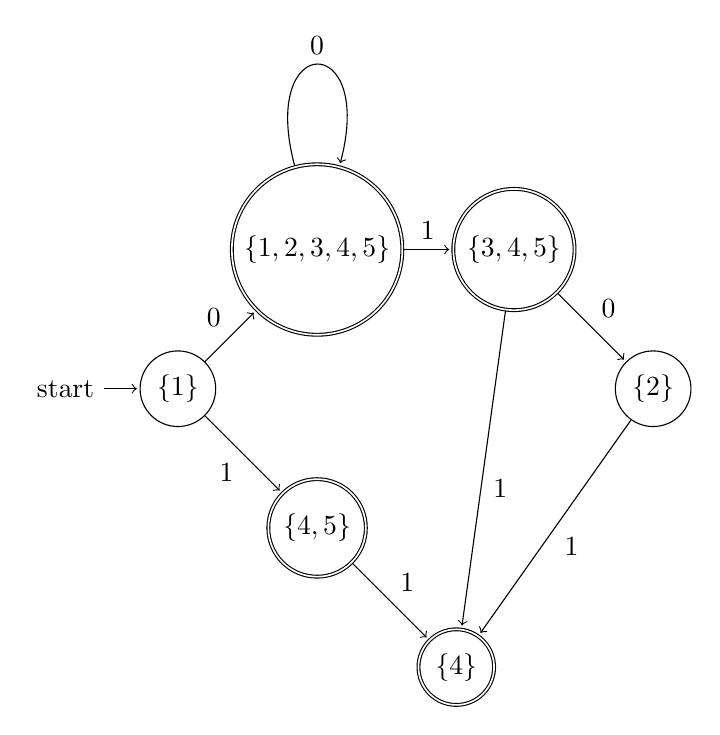
\begin{tikzpicture}[shorten >=1pt,node distance=2.5cm,on grid,auto] 
   \node[state,initial] (q_0)   {$\{1\}$}; 
   \node[state,accepting] (q_1) [above right=of q_0] {$\{1,2,3,4,5\}$}; 
   \node[state,accepting] (q_2) [below right=of q_0] {$\{4,5\}$}; 
   \node[state,accepting] (q_3) [right=of q_1] {$\{3,4,5\}$};
   \node[state,accepting] (q_4) [below right=of q_2] {$\{4\}$};
   \node[state] (q_5) [below right=of q_3] {$\{2\}$};
    \path[->] 
    (q_0) edge  node {0} (q_1)
          edge  node [swap] {1} (q_2)
    (q_1) edge  node  {1} (q_3)
          edge [loop above] node {0} ()
    (q_2) edge node {1} (q_4)
    (q_3) edge node {1} (q_4)
          edge node {0} (q_5)
    (q_5) edge node {1} (q_4);
\end{tikzpicture}
\end{enumerate}

\section{Question 2}

\begin{enumerate}[leftmargin=\labelsep]
\item[2.1] TODO


\item[2.2]


\item[2.3]

\end{enumerate}

\section{Question 3}

\begin{enumerate}[leftmargin=\labelsep]

\item[3.1]

\item[3.2]

\end{enumerate}

\end{document}
